\section{Strategies for Subtitles Positioning in 360° Video}
\label{sec:subtitles}
We searched for works that used strategies for subtitles positioning in the last 5 years, and extracted the strategies they presented, also described as subtitling behaviour~\cite{brown_subtitles_2017}, in 360-degree videos. Then, we merged the similar strategies and divided them into three main categories: \emph{screen-referenced subtitles}, \emph{world-referenced subtitles} and \emph{dynamic subtitles}. Each of these categories are described in Subsections \ref{subsec:screen_referenced}, \ref{subsec:world_referenced}, and \ref{subsection:dynamic_subtitles} respectively. Table \ref{tab:catalog} contains a summary about the strategies in each category, their advantages and disadvantages.

\begingroup
%\renewcommand{\baselinestretch}{1.5}
\begin{table}[!ht]
\footnotesize
\caption{Subtitles positioning strategies catalog for 360-degree video}
\label{tab:catalog}
\hspace{-1em}
\begin{tabular}{@{}llll@{}}
\toprule
\textbf{Category}                                               & \textbf{Strategy}  & \textbf{Advantages}                                                                                    & \textbf{Disadvantages}                                                                                         \\ \midrule
\multicolumn{1}{c}{\multirow{2}{*}{\textbf{Screen-Referenced}}} & Static-Follow      & \begin{tabular}[c]{@{}l@{}}easy to locate;\\ freedom of movement;\\ most common strategy;\end{tabular} & issues with nausea;                                                                                            \\ \cmidrule(l){2-4} 
\multicolumn{1}{c}{}                                            & Lag-Follow         & \begin{tabular}[c]{@{}l@{}}issues with nausea mitigated\\ in comparison to static-follow;\end{tabular} & may cause rereading;                                                                                           \\ \midrule
\multirow{2}{*}{\textbf{World-Referenced}}                      & Repeated Subtitles & \begin{tabular}[c]{@{}l@{}}comfort;\\ could be ``burnt-in'' the video;\end{tabular}                    & \begin{tabular}[c]{@{}l@{}}may cover important content;\\ may be confusing;\\ not always visible;\end{tabular} \\ \cmidrule(l){2-4} 
                                                                & Appear             & \begin{tabular}[c]{@{}l@{}}comfort;\\ subtitles can be ``dismissed";\end{tabular}                      & \begin{tabular}[c]{@{}l@{}}may be positioned in spurious\\ locations;\\ not always visible;\end{tabular}       \\ \midrule
\textbf{Dynamic}                                                & Speaker-Following  & help in speaker identification;                                                                        & not always visible;                                                                                            \\ \bottomrule
\end{tabular}
\end{table}
\endgroup

\subsection{Screen-Referenced Subtitles}
\label{subsec:screen_referenced}
In this category, the subtitles are positioned taking the screen as reference, which can also be the viewport in a HMD. The subtitles basically follow the user's view and can be seen at any instant of time. We have identified two strategies following this category: \emph{static-follow} and \emph{lag-follow}. Each of these strategies are describe in Subsections \ref{subsubsec:static_follow} and \ref{subsubsec:lag_follow}, respectively.

\subsubsection{Static-Follow}
\label{subsubsec:static_follow}

When defining the \emph{static-follow} strategy, \citeonline{brown_subtitles_2017} argue that it is a common behaviour for showing information in Virtual Reality~(VR) experiencies, as part of a ``head-up display'' (HUD). A HUD typically displays graphics that are fixed in front of the viewer at all times regardless of their posture and pose in a VR environment. Figure \ref{fig:static_follow} shows this strategy, which uses the aforementioned HUD mechanic. In this strategy, the subtitles are shown to the viewer as if they were static relative to their head, by following the viewer as they look around the environment. The subtitles are placed 15º vertically bellow eye-level. \citeonline{brown_subtitles_2017} mention that a possible caveat of this strategy is that some works have reported that overuse of HUD can cause issues, such as nausea \cite{laviola2000discussion, sharples2008virtual}.

The work of \citeonline{meira_video_2016} uses this strategy for subtitles positioning. The authors mention that the subtitles are presented at the botton of the user's viewport and follow their gaze, but they do not mention how many degrees bellow eye-level are used. The work of \citeonline{matos_dynamic_2018} investigates the use of dynamic annotations in 360-degree video, with subtitles being one kind of such annotations. The authors mention the work of \citeonline{brown_subtitles_2017} and call the \emph{static-follow} strategy by \emph{persistent}, in which subtitles~(annotations) are placed in front of the user's view. \citeonline{rothe_dynamic_2018} refer to this strategy as \emph{static subtitles}, and say that, in a study they conducted, this was the preferred strategy among the ones proposed by \citeonline{brown_subtitles_2017}. They also mention that the subtitles were positioned at 12.5º bellow eye-level. The work of \citeonline{hughes_disruptive_2019} refers to this strategy as \emph{fixed position in the display picture} and mentions that it is the most common way of using subtitles in 360-degree video. Finally, \citeonline{montagud_culture_2020} says that there is a follow-up on the work \citeonline{brown_subtitles_2017} that refers to this strategy as \emph{folow head immediately}. In this follow-up work (a white paper), \citeonline{brown2018exploring} evaluate the four strategies proposed in \citeonline{brown_subtitles_2017}. %Such white paper was not included in our SLR since it is a non-peer reviewed work.

\begin{figure}[!ht]
    \centering
    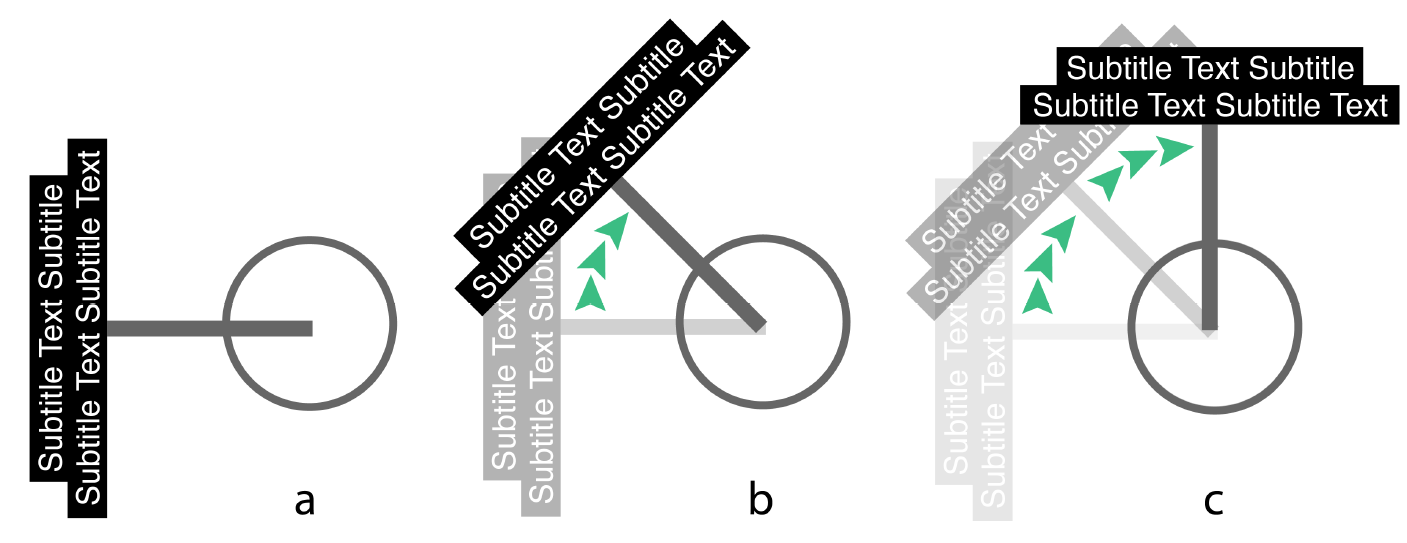
\includegraphics[width=0.7\textwidth]{img/static-follow.png}
    \caption{Static-Follow: The sequence a, b, c demonstrates how as the user turns their head, the subtitles stay fixed to the centre of their field of view. Extracted from the work of Brown et al. (2017).}
    \label{fig:static_follow}
\end{figure}




\subsubsection{Lag-Follow}
\label{subsubsec:lag_follow}

\citeonline{brown_subtitles_2017} define the \emph{lag-follow}~(see Figure \ref{fig:lag_follow}) stategy to address the sicknes related to the \emph{static-follow} strategy while still keeping the subtitles visible to the viewer. Similar to the \emph{static-follow} strategy, the subtiles appear in front of the viewer. It remains in such posititon~(relative to the environment) until the viewer's head rotates more than the 30º threshold. The subtitles then smoothly rotates to be in front of the viewer again. It is worth noticing that the subtitles can only move along the horizontal axis. The main objective of this strategy is to provide freedom of movement to the viewer without immediate reaction from subtitles. \citeonline{brown_subtitles_2017} say, however, that this strategy may cause the viewer to reread the subtitles, which is not desirable.


\begin{figure}[!ht]
    \centering
    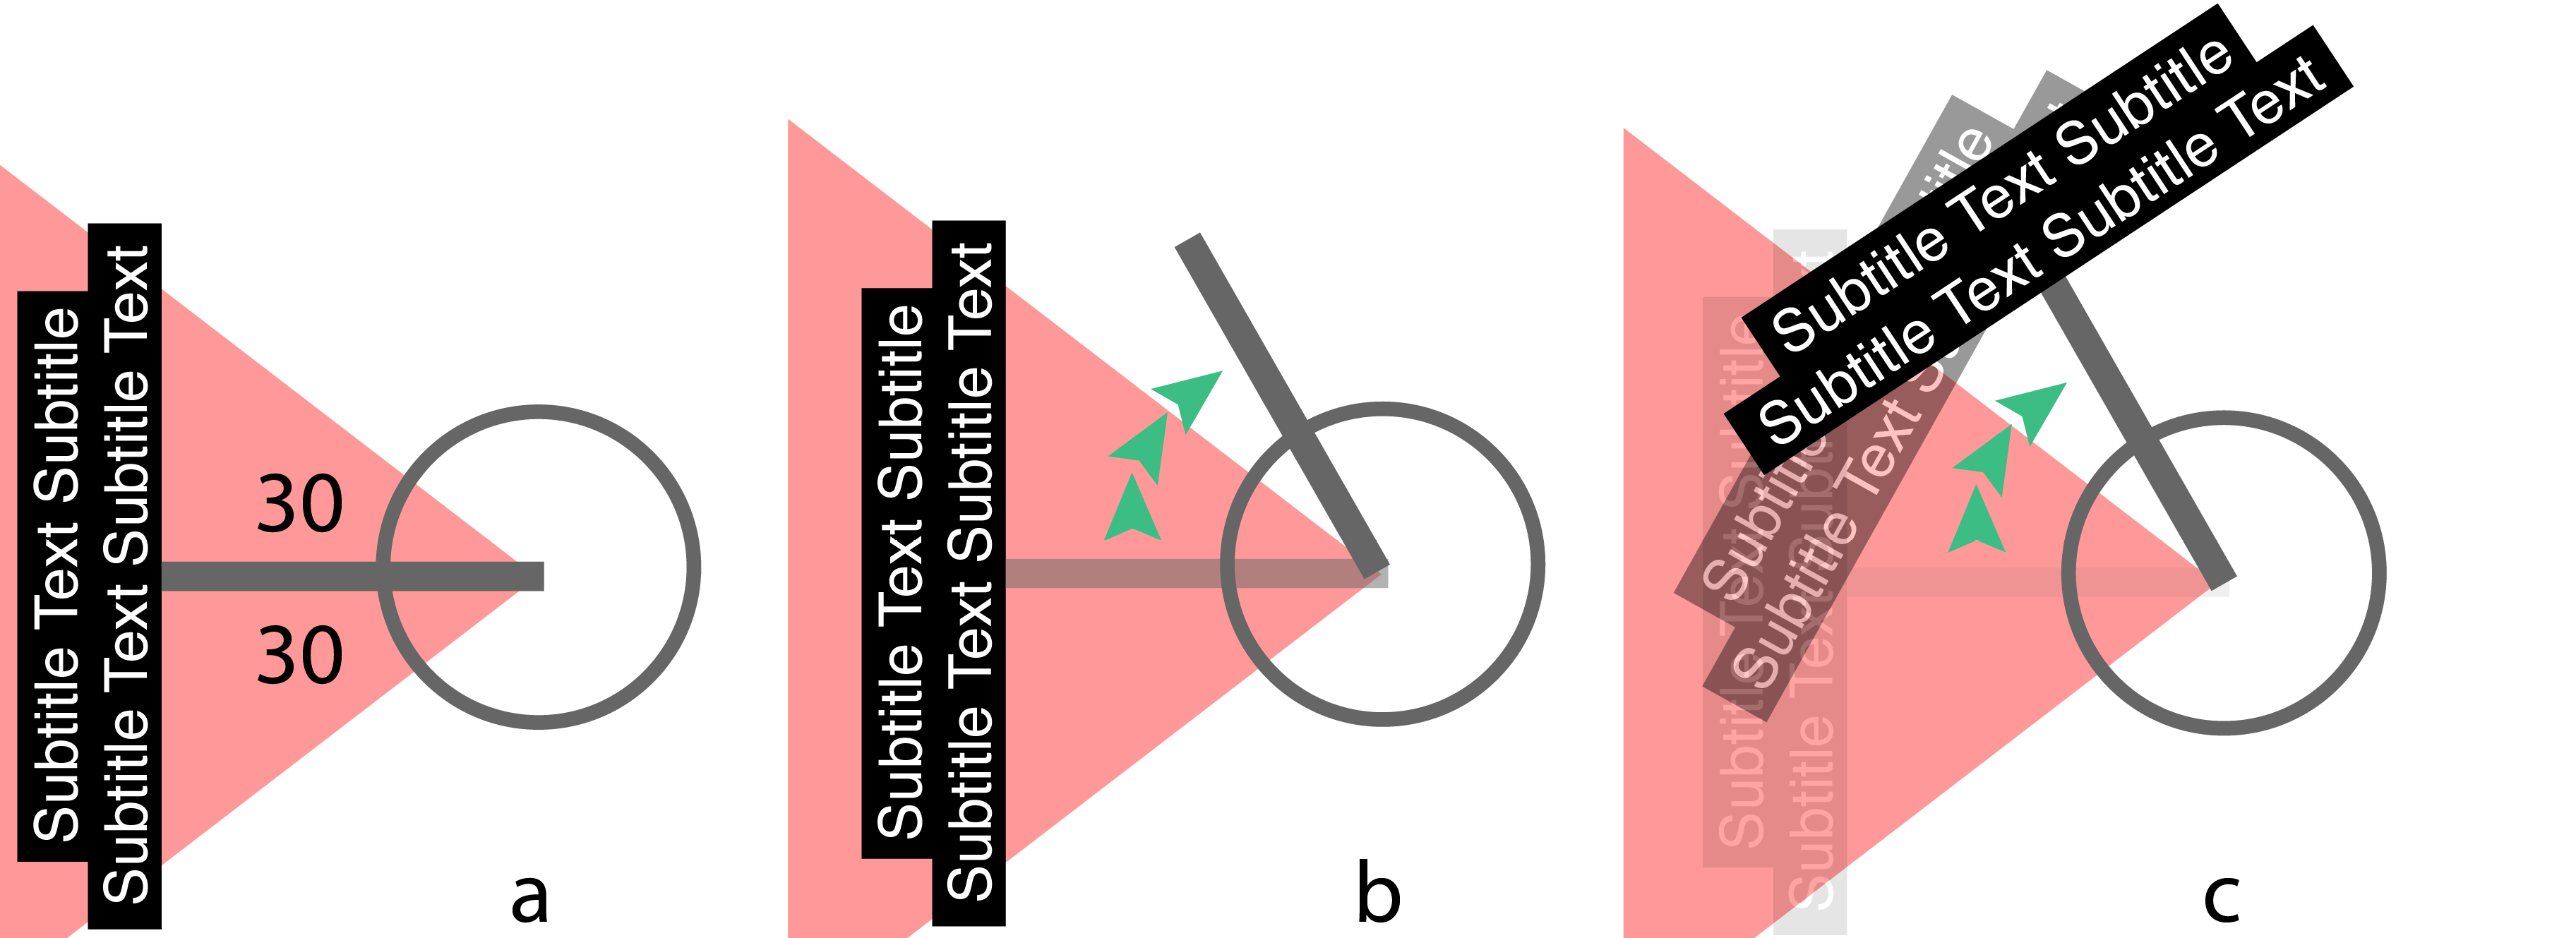
\includegraphics[width=0.7\textwidth]{img/lag-follow.png}
    \caption{Lag-Follow: a. Small user head movements ($<30^{\circ}$) are ignored. b. But turning beyond this boundary c. The subtitles move smoothly to the center of the field-of-view. Extracted from the work of Brown et al. (2017).}
    \label{fig:lag_follow}
\end{figure}

The work of \citeonline{matos_dynamic_2018} describes a strategy that is basically the same of this one. It is called \emph{floating}, it starts in a position and floats into the viewer's field-of-view. Similar to what was descibed in Subsection \ref{subsubsec:static_follow}, the work of \citeonline{montagud_culture_2020} refers to this strategy with a different name (\emph{follow with lag}), but having the same definition.

\subsection{World-Referenced Subtitles}
\label{subsec:world_referenced}
In this category, the subtitles are positioned by taking the 360 environment as reference. 
As referenced in \cite{hughes_disruptive_2019}, this category of strategy leads to better results in comfort~\cite{rothe2018positioning}. \citeonline{rothe2018positioning}, as referenced in \citeonline{hughes_disruptive_2019}, also say that world-referenced subtites conflict, in general, with the requirement that a user must always be able to read the subtitle text because it limitates the user's freedom of exploring the scene.
We have identified two strategies following this category: \emph{repeated subtitles} and \emph{appear subtitles}. These strategies are described in Subsections \ref{subsubsection:repeated_subtitles} and \ref{subsubsection:appear_subtitles}, respectively. 

\subsubsection{Repeated Subtitles}
\label{subsubsection:repeated_subtitles}

In this strategy, repeated subtitles are place around the user. These subtitles stay fixed in the environment and do not follow the user's head motion. Figure \ref{fig:120_subtitles} shows three repeated subtitles evenly spaced by angles of 120°. Such figure was extracted from the work of \citeonline{brown_subtitles_2017}. The authors argue that one of the main advantages of this strategy for subtitles positioning is that the subtitles could be ``burnt-in'' to the video using a video-editor. This strategy is refered as \emph{120-degree} in the work of \citeonline{brown_subtitles_2017}, and as \emph{evenly spaced} in the work of \citeonline{montagud_culture_2020}. A caveat of this strategy, mentioned by \citeonline{brown_subtitles_2017}, is that it may cover important content located in unfortunate positions. 

\citeonline{li_impacts_2018} use this strategy to evaluate the impacts of subtitles in 360-degree video journalism. They do not evaluate the subtitles positioning itself, but the impact of the subtitles. The work of \citeonline{chen_film_2017} uses this strategy for positioning subtitles while investigating film language in society news using 360-degree videos of The New York Times. During their study, some participants found the \emph{repeated subtitles} strategy confusing as they thought, in some moments, that the subtitles in different positions had different text.

\begin{figure}[!ht]
    \centering
    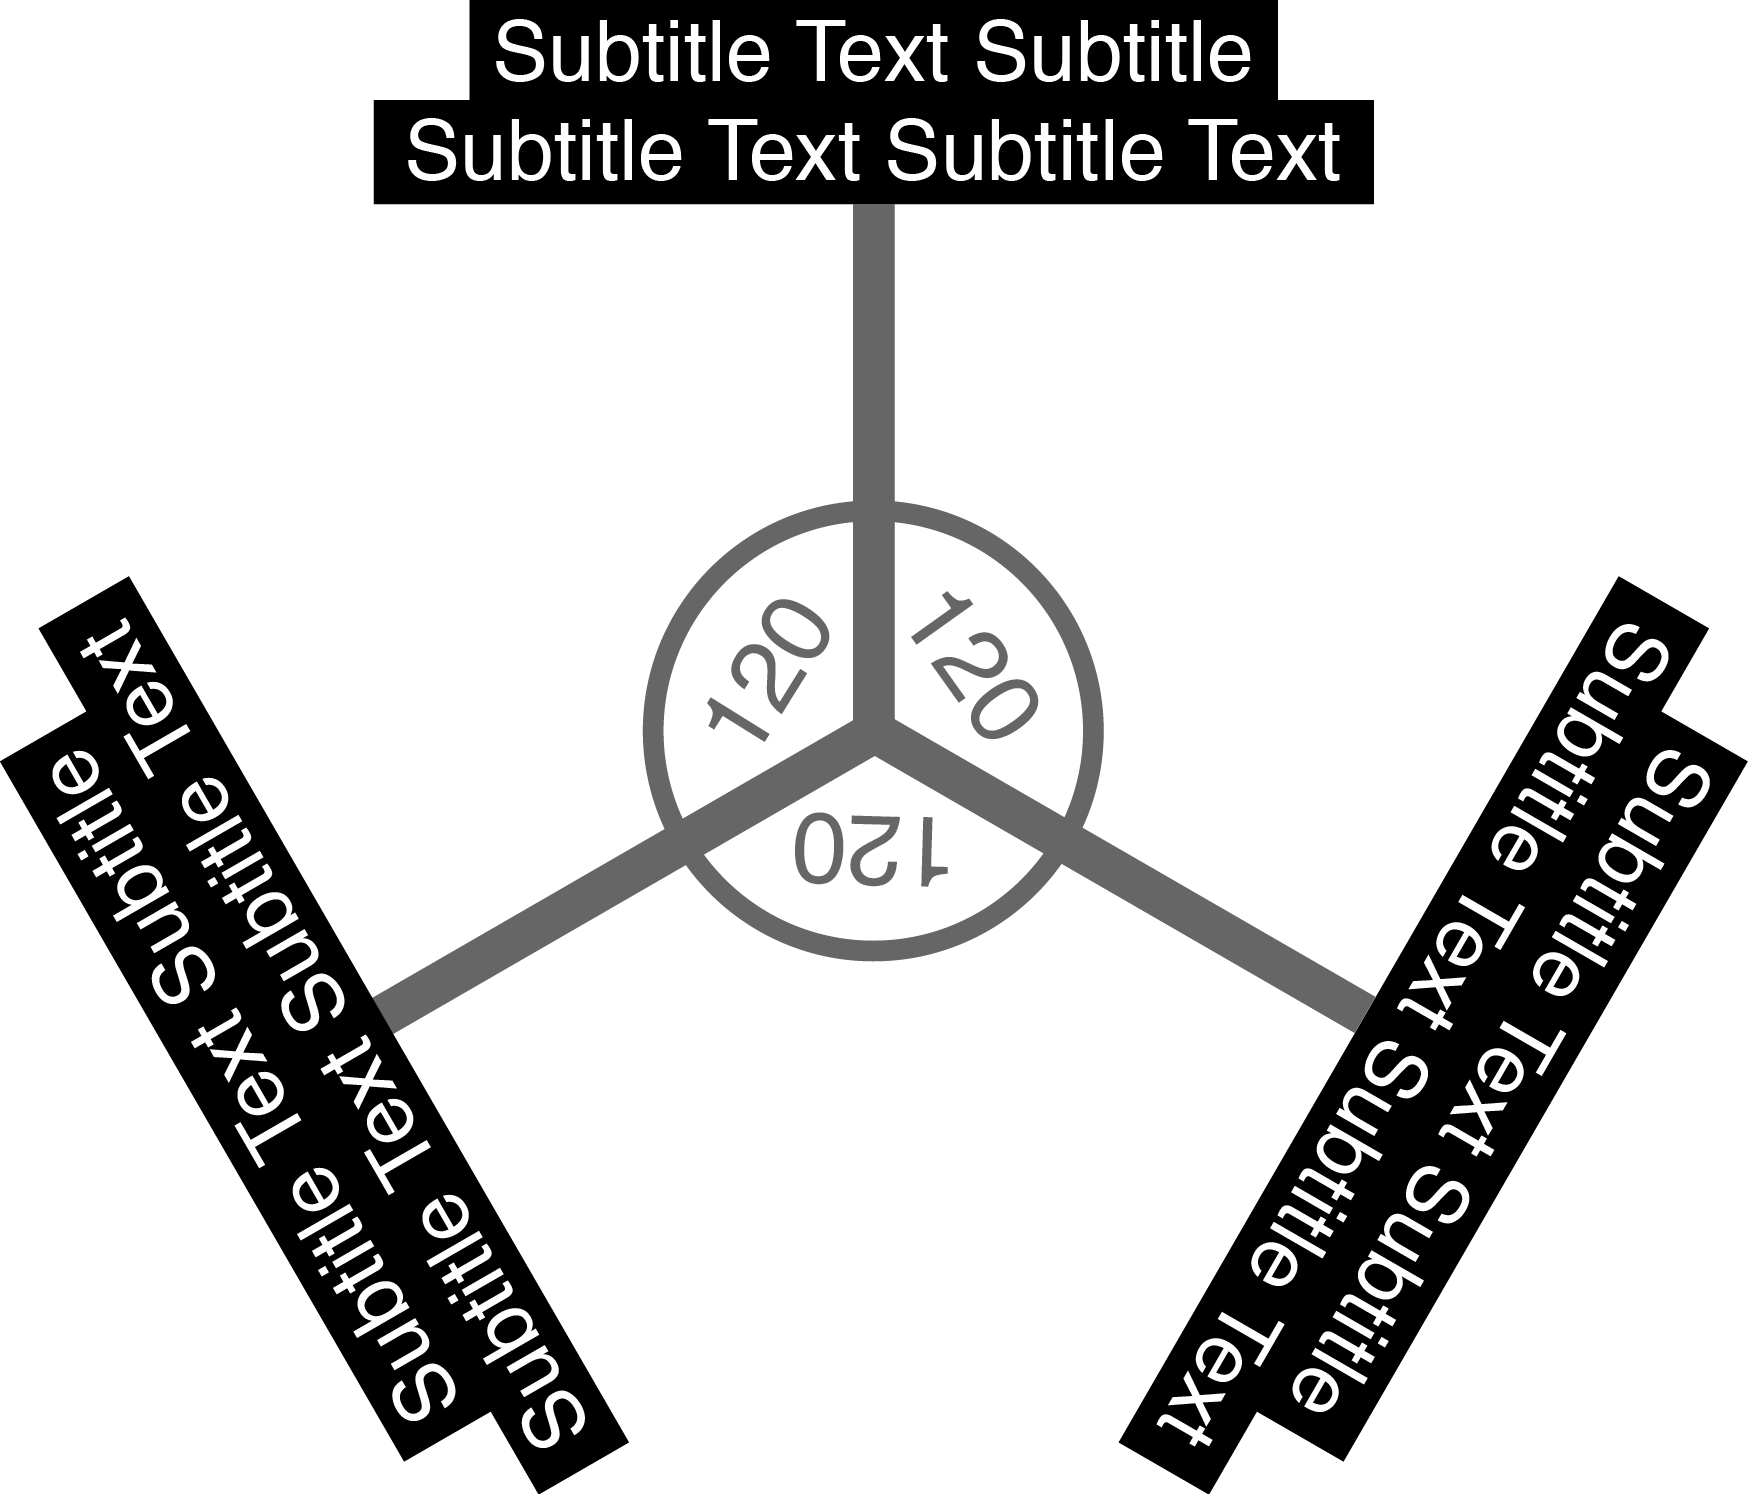
\includegraphics[width=0.35\textwidth]{img/120_subtitles.png}
    \caption{Three repeated subtitles (having the same text) are located in the environment at 120° angles around the viewer. Extracted from the work of Brown et al. (2017).}
    \label{fig:120_subtitles}
\end{figure}

\subsubsection{Appear Subtitles}
\label{subsubsection:appear_subtitles}

\citeonline{brown_subtitles_2017} say that, based on feedback from a user whom was hard of hearing, they had the idea of creating a strategy in which the viewer can dismiss the subtitle after reading it. From that feedback, they designed the \emph{appear} strategy. As it is depicted in Figure \ref{fig:appear_subtitle}, the subtiles are placed at the centre of the user's field of view horizontally, 15º bellow eye-level. If the viewer moves their head, the subtitles remain static within the environment and do not follow their gaze. This strategy is also referenced as \emph{appear in front, then fixed} in the work of \citeonline{montagud_culture_2020}. A possible caveat of this strategy, mentioned by \citeonline{brown_subtitles_2017}, is that the subtitles may be positioned in spurious locations if the viewer is quickly moving their head.

\begin{figure}[!ht]
    \centering
    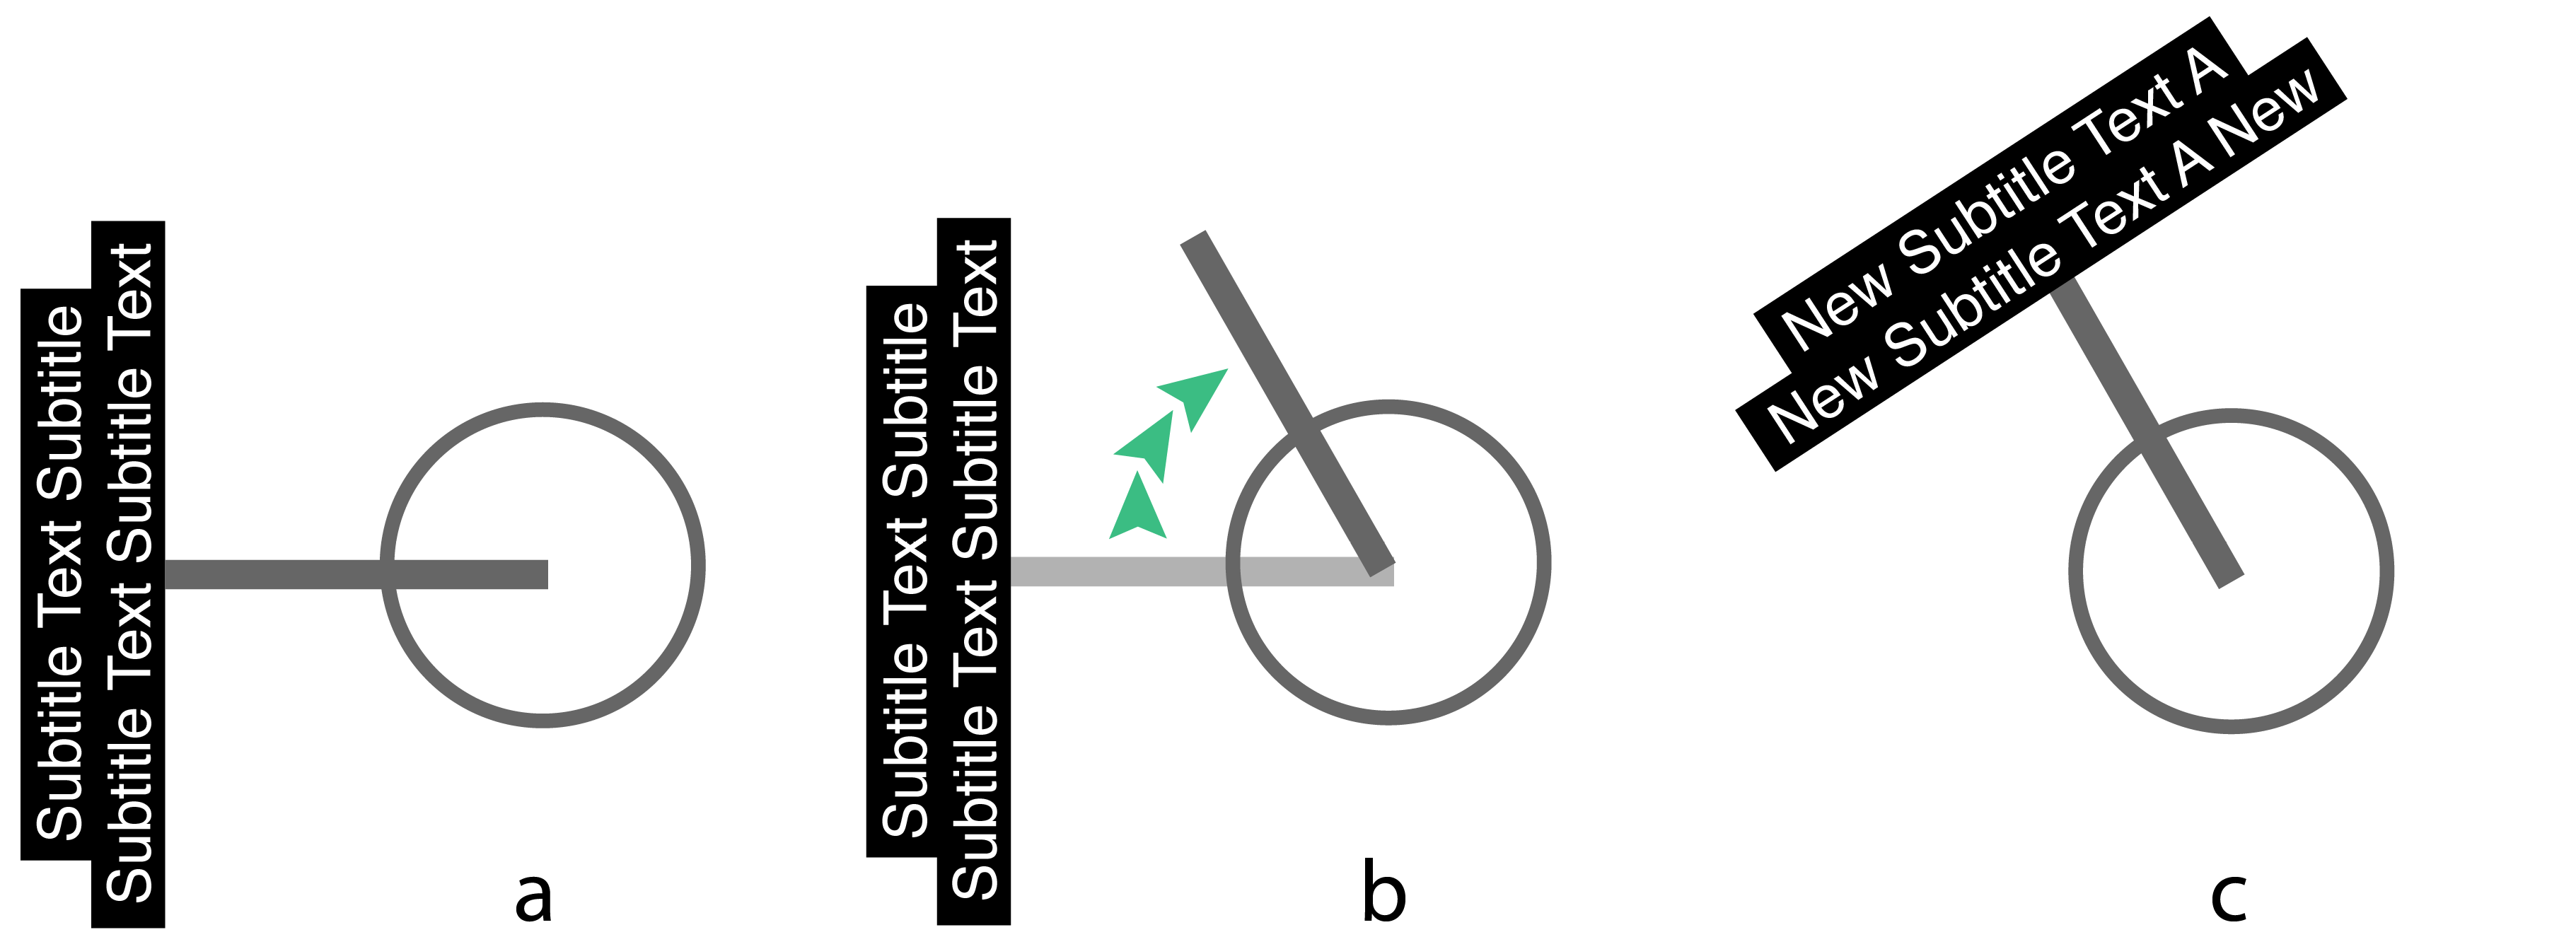
\includegraphics[width=0.7\textwidth]{img/appear.png}
    \caption{Appear: a. A subtitle appears at the centre of the user's view. b. If the user moves before the subtitle is due to change, it will remain static in the environment. c. When a new subtitle is shown, it will appear at the centre of the user's view again. Extracted from the work of Brown et al. (2017).}
    \label{fig:appear_subtitle}
\end{figure}

\subsection{Dynamic Subtitles}
\label{subsection:dynamic_subtitles}

In this category, the position of subtitles dinamically changes and depends on the scene \cite{rothe_dynamic_2018}. As referring to annotations~(that could be subtitles), \citeonline{matos_dynamic_2018} say that there are cases where the point of interest is moving through the video, which requires a dynamic annotation that follows its movement. One strategy that we have identified in this category is the \emph{speaker-following subtitles} strategy, described in \ref{subsubsec:speaker_following}.

\subsubsection{Speaker-Following Subtitles}
\label{subsubsec:speaker_following}

In this strategy, the subtitles are placed close to the speaker~(see Figure \ref{fig:speaker_following}). Since the speakers may move during the video, this strategy fits in the \emph{dynamic subtitles} category. This strategy also helps in the issue of \emph{speaker identification}, as all persons in the room are visible in a 360-degree video~\cite{rothe_dynamic_2018}.  

\citeonline{rothe_dynamic_2018} compared \emph{speaker-following} subtitles with the \emph{static-follow} strategy regarding task workload, simulator sickness and presence. For evaluating each of these dimensions, the authors used, respecively, the following questionaires: NASA-TLX~\cite{nasa_hart1988development}; Simulator Sickness Questionaire~\cite{sickness_kennedy1993simulator}; and Presence Questionaire~\cite{presence_witmer1998measuring}. When asking which strategy the participants preferred, the authors received balanced answers. However, \emph{speaker-following} subtitles led to higher score of presence, less sickness and lower workload~\cite{rothe_dynamic_2018}.

\begin{figure}[!ht]
    \centering
    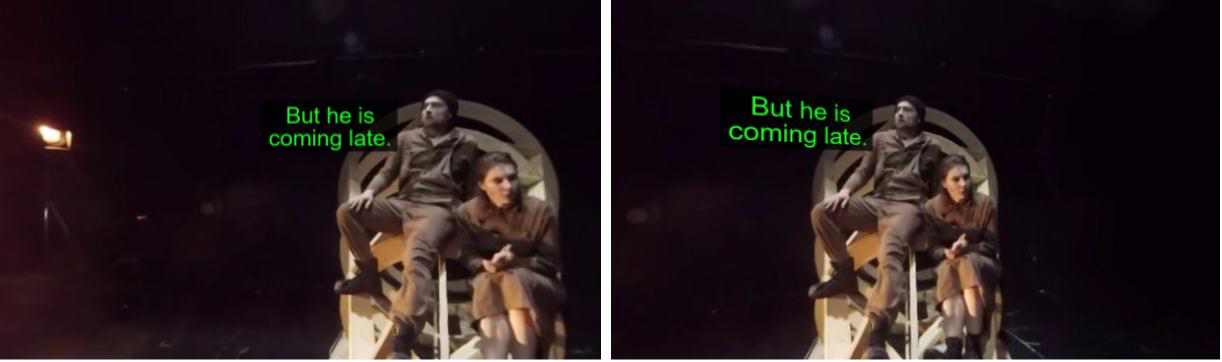
\includegraphics[width=0.85\textwidth]{img/speaker-following.png}
    \caption{Speaker-following subtitles. Extracted from the work of Hughes et al. (2019).}
    \label{fig:speaker_following}
\end{figure}
